% Compile broadcast.tex / connection.tex with XeLaTeX.
\documentclass[tikz,border=7mm]{standalone}
\usepackage{fontspec}
\usepackage{xeCJK}
\usepackage{graphicx}
\setmainfont{texgyreheros-regular.otf}[BoldFont=texgyreheros-bold.otf]
\setCJKmainfont{FandolHei-Regular.otf}[BoldFont=FandolHei-Bold.otf]
\usetikzlibrary{calc,arrows.meta}
\definecolor{ink}{HTML}{233247}
\definecolor{muted}{HTML}{697586}
\definecolor{lan}{HTML}{3173B9}
\definecolor{lanfill}{HTML}{F1F7FD}
\definecolor{outline}{HTML}{B8C8D8}
\definecolor{roomfill}{HTML}{F8FAFC}
\begin{document}
\begin{tikzpicture}[text=ink,font=\normalsize,
 cable/.style={draw=lan,line width=1.15pt,line cap=round,line join=round,rounded corners=2mm}]
 \path[use as bounding box] (-3.05,-3.15) rectangle (10.25,6.55);
 \node[font=\LARGE\bfseries] at (3.6,6.15) {\diagramtitle};
 % Cables start at actual sockets on the underside of each computer.
 \draw[cable] (1.5,-.35) -- (1.5,-2.25) -- (2.15,-2.25);
 \ifdefined\connected
  \draw[cable] (5.05,-2.25) -- (5.7,-2.25) -- (5.7,-.35);
  \draw[cable,-{Stealth[length=3mm,width=2.4mm]}] (5.7,-1.9) -- (5.7,-1.25);
  \draw[cable,-{Stealth[length=3mm,width=2.4mm]}] (1.5,-1.05) -- (1.5,-1.7);
  \node[font=\small,text=lan,anchor=west,inner sep=0] at (1.85,-1.3) {NDI 流};
  \node[font=\small,text=lan,anchor=east,inner sep=0] at (5.35,-1.3) {NDI 流};
 \else
  \draw[cable] (5.05,-2.25) -- (5.7,-2.25) -- (5.7,-.35);
 \fi
 \node[font=\small,text=muted,anchor=east,inner sep=0] at (1.15,-1.6) {网线};
 \node[font=\small,text=muted,anchor=west,inner sep=0] at (6.05,-1.6) {网线};
 \filldraw[fill=lanfill,draw=lan,line width=.9pt,rounded corners=2.5mm]
  (2.15,-2.82) rectangle (5.05,-1.68);
 \node[font=\large\bfseries] at (3.6,-2.25) {有线局域网};
 \foreach \x/\role/\action in {0/发送端/发送,7.2/接收端/接收} {
  \node[font=\large\bfseries] at (\x,5.18) {\role};
  \node[font=\small,text=muted] at (\x,4.7) {OBS DistroAV \action};
  % Stand is drawn first so the monitor housing cleanly conceals its top edge.
  \filldraw[fill=roomfill,draw=outline,line width=.8pt]
   (\x-.25,-.9) rectangle (\x+.25,-.16);
  \filldraw[fill=roomfill,draw=outline,line width=.8pt,rounded corners=.7mm]
   (\x-.9,-1.02) rectangle (\x+.9,-.87);
  \filldraw[fill=roomfill,draw=outline,line width=.85pt,rounded corners=2mm]
   (\x-2.8,-.35) rectangle (\x+2.8,4.22);
  % Full 4:3 image viewport, exact aspect ratio, with a restrained inner border.
  \fill[white] (\x-2.6,.12) rectangle (\x+2.6,4.02);
  \draw[outline,line width=.35pt] (\x-2.6,.12) rectangle (\x+2.6,4.02);
 }
 \ifdefined\connected
  \node[inner sep=0] at (0,2.07) {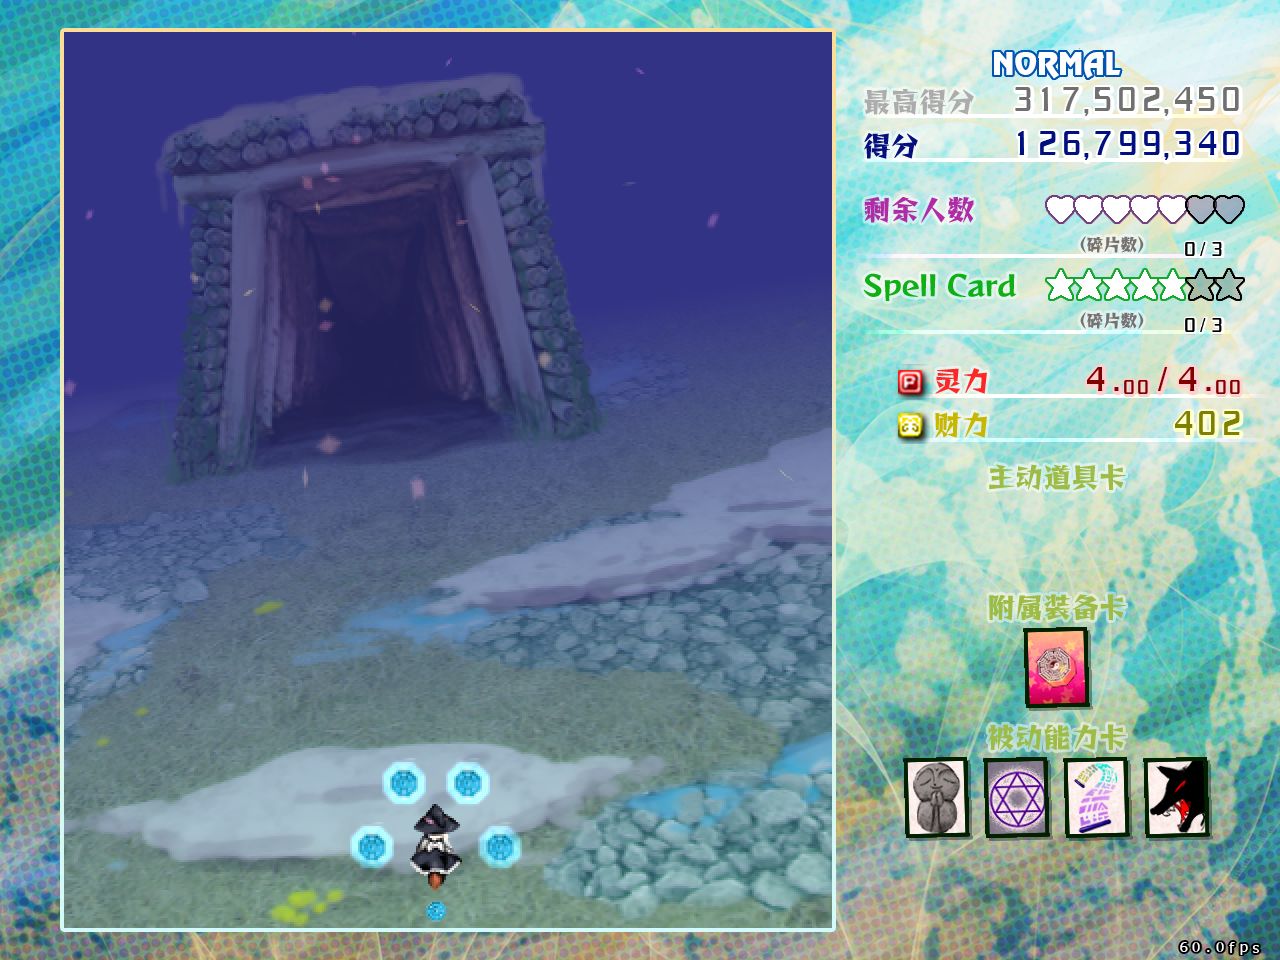
\includegraphics[width=5.2cm]{assets/gameplay.png}};
  \fill[black] (4.6,.12) rectangle (9.8,4.02);
  \node[text=white,font=\footnotesize,inner sep=0] at (7.2,.47) {OBS NDI 源\enspace 推流接收中…};
  \node[inner sep=0] at (7.2,2.21) {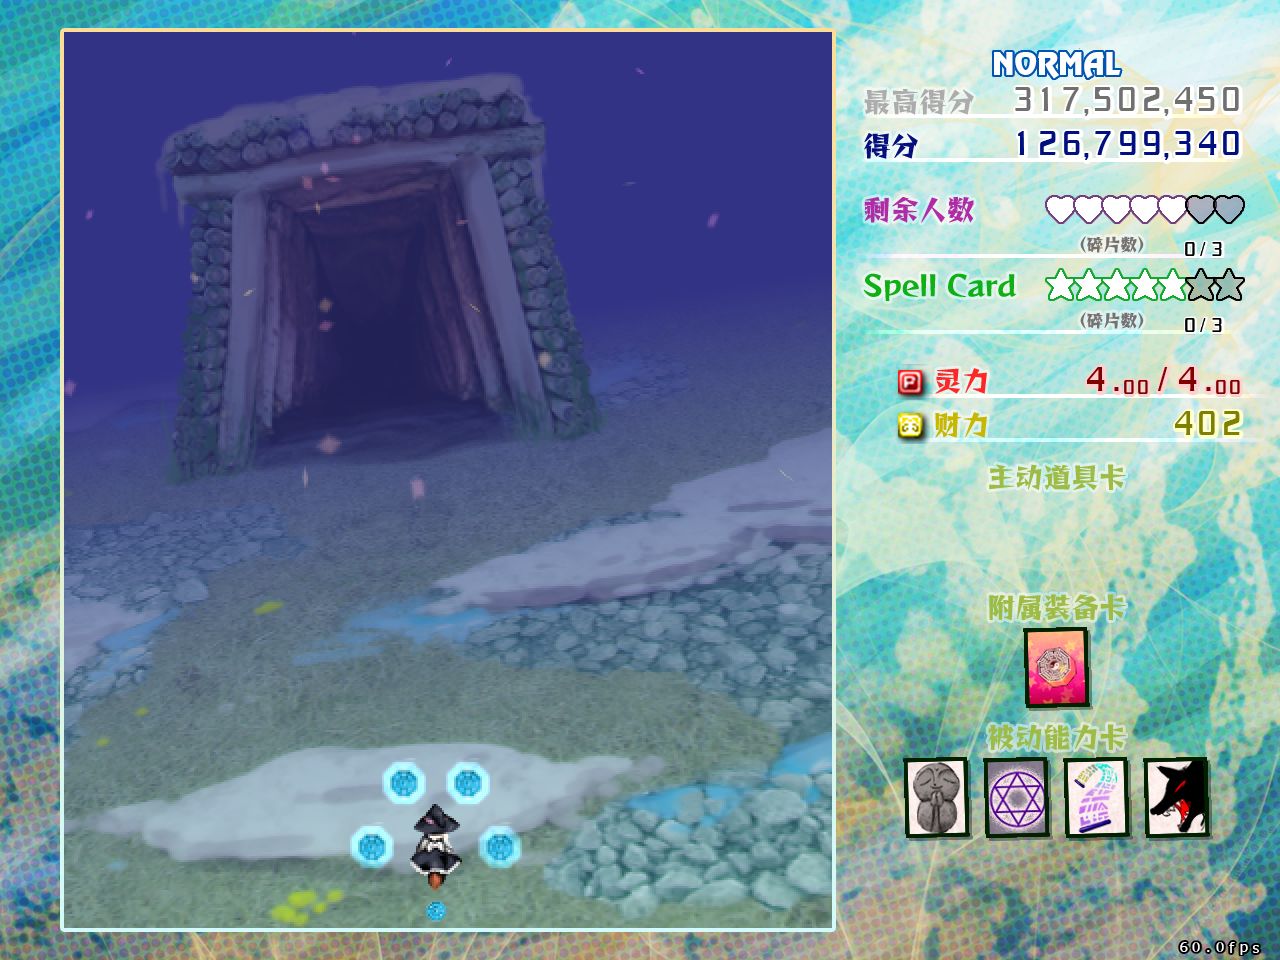
\includegraphics[width=3.8cm]{assets/gameplay.png}};
 \else
  \node[inner sep=0] at (0,2.07) {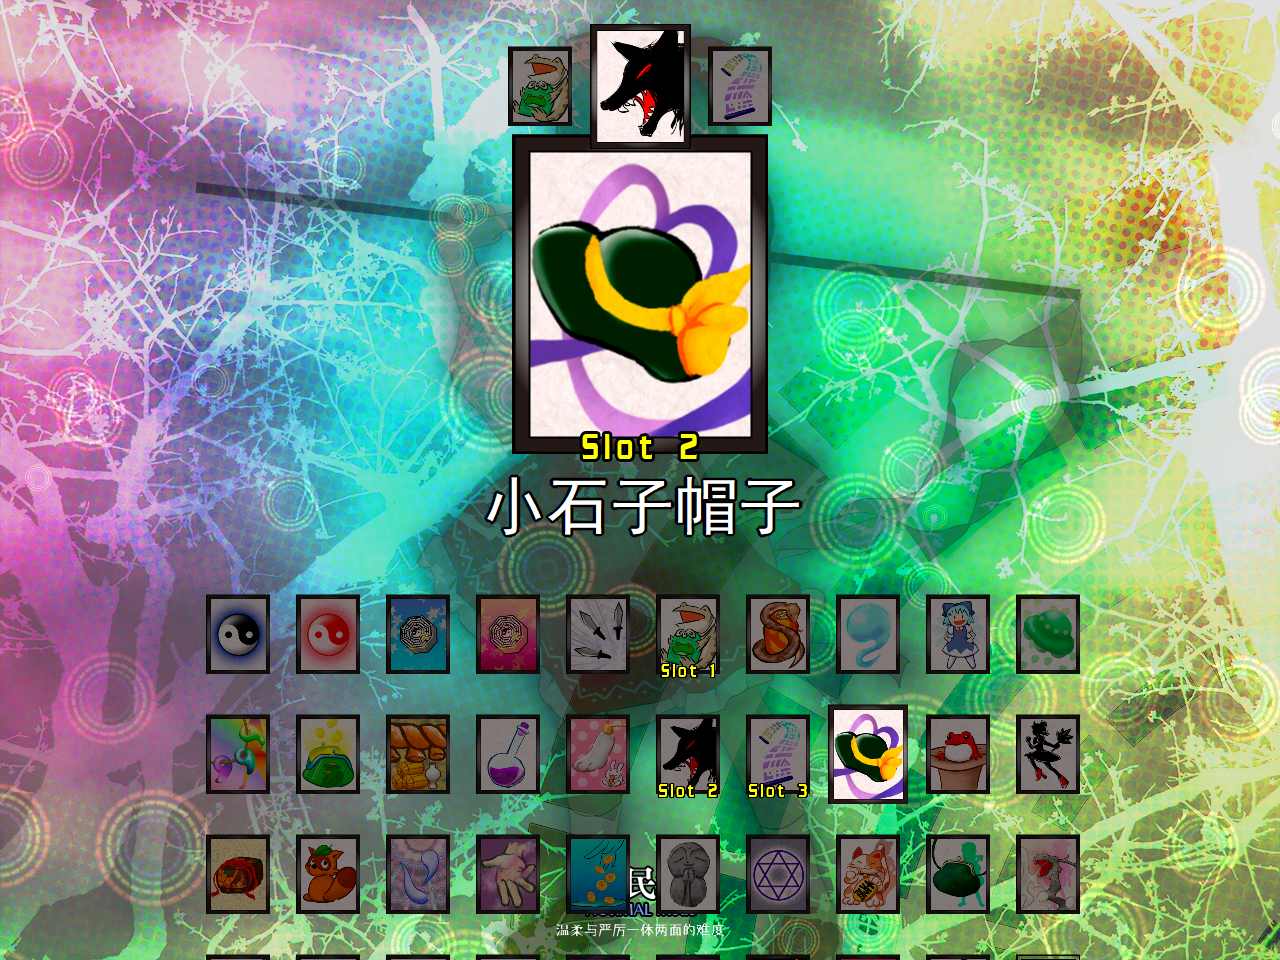
\includegraphics[width=5.2cm]{assets/discovery.png}};
  % Availability belongs to the computer, not the captured game screen.
  \fill[lan] (-.7,-.115) circle[radius=.65mm];
  \node[font=\footnotesize,text=lan,anchor=west,inner sep=0] at (-.53,-.115) {可被发现};
  \node[anchor=west,font=\small,text=muted,inner sep=0] at (5.05,2.64) {来源名称：};
  \filldraw[fill=lanfill,draw=outline,line width=.65pt,rounded corners=1mm]
    (5.05,1.55) rectangle (9.35,2.23);
  \node[anchor=west,font=\normalsize,inner sep=0] at (5.25,1.89) {OBS-发送端};
  \draw[lan,line width=.7pt] (8.93,1.97) -- (9.03,1.87) -- (9.13,1.97);
 \fi

 % Connection sockets meet the cable ends without crossing the stands.
 \foreach \x in {1.5,5.7} {
   \filldraw[fill=white,draw=lan,line width=.65pt] (\x,-.35) circle[radius=1.1mm];
 }
\end{tikzpicture}
\end{document}
